\documentclass[journal]{IEEEtran}

\usepackage{graphicx}
\usepackage{url}
\usepackage{cite}
\usepackage{amsmath}
\usepackage{algorithmic}
\usepackage{amssymb}
\usepackage{hyperref}
\usepackage{listings}

\hyphenation{op-tical net-works semi-conduc-tor}


\begin{document}
\title{Simplifying Meta-Beamforming Algorithms for Massive Wireless Networks}

\author{Cameron~Kramr}

% The paper headers
\markboth{Rice University, RCEL 576, Final Project. December 2023}{}

% make the title area
\maketitle

\begin{abstract}
Machine learning in wireless communications has helped to solve many important issues related to next generation wireless systems. One major issue encountered by modern communication system is related to spatial multiplexing and reducing interference caused by neighboring users \cite{Through_Max}. To reduce this interference, modern systems use electronic beamforming to direct the radiation pattern of each user away from every other user while maintaining contact with the base-station \cite{Intelligent_mMMIMO}. The optimal solution to this problem is an NP-hard Minimal Mean Squared Error (MMSE) optimization problem with a slow response time that needs to be recalculated as the users move and the channel properties changes \cite{NO_inverse_MMSE}. To get around this, Deep Neural Networks (DNNs) have been deployed at various levels to either estimate the end-to-end problem, or to estimate certain difficult portions of the original computation \cite{Review_DL_BF}. This paper attempted to improve upon the architecture presented in \cite{LSTM_Net} to reduce the computational complexity of calculating the optimal beam forming weights by using a GRU based architecture instead of an LSTM. While implementation details combined with an insufficiently documented source prevented further exploration, a great deal was learned about deploying neural networks in a reinforcement learning setting. 
\end{abstract}


%-------------------------------------------------------------------------------
%                          Introduction
%-------------------------------------------------------------------------------
\section{Introduction}
\IEEEPARstart{T}{he} coming Industry 4.0 requires high-density wireless device connectivity with high-throughput \cite{Through_Max}. High data-throughput requires large amounts of bandwidth, but bandwidth used by one device cannot be used by others. To mitigate this, traditional networks deploy time and frequency domain multiplexing \cite{Through_Max}. These solutions allocate finite time and frequency between different users, and so through-put collapses as the number of users increases. To solve the problem of finite time and frequency, 5th generation networks apply spatial multiplexing which allows multiple users to share time and frequency and not interfere with each other \cite{Through_Max, Intelligent_mMMIMO}. Spatial multiplexing is performed by electrically shaping the beam of an array of antennas toward its target and away from other users \cite{Intelligent_mMMIMO}. Beam-forming requires calculating weights and phase delays for a spatial array of antennas so that radiation goes mostly where desired and avoids undesired places \cite{lu2020learningbased}, \cite{Review_DL_BF}, \cite{How_many_ant}.  

The problem of optimizing antenna weights so that radiation reaches its target and avoids interfering with other users is NP-Hard \cite{MMSE_Apps}. Modern communications systems solve for the optimal weights using the Minimal Mean Squared Error method \cite{MMSE_Apps}. Because the MMSE method is iterative, the algorithm adapts slowly to changing environments which is unacceptable for mobile communications networks. To mitigate the slow response of the optimal solution, many sub-optimal approximations and other optimizations have been explored \cite{Iteratively_MMSE}. One optimization that shows promise is deploying Deep Neural Networks (DNNs) to approximate the antenna weights in dense networks \cite{Review_DL_BF}. State of the art beam-forming networks deploy DNNs either in end-to-end configurations, or to approximate difficult portions of the MMSE algorithm \cite{Review_DL_BF}. 

The paper \cite{LSTM_Net} implemented an LSTM to decrease the computation required to find optimal antenna weights. The authors of \cite{LSTM_Net} used an LSTM network to learn how to optimize the parameters of the optimization problem in a method that will be discussed later in the paper. The method of using LSTMs is the state of the art method for finding optimal antenna weights \cite{Review_DL_BF, LSTM_Net}. This paper attempted to reduce the computation required to find antenna weights further using a simpler recurrent architecture, the Gated Recurrent Unit GRU and to document the process of training this architecture. This remains open work since this project was unable to properly replicate results of \cite{LSTM_Net, Review_DL_BF, NO_inverse_MMSE, Intelligent_mMMIMO}. The remainder of this paper will discuss in detail the exact optimization method attempted in the background and prior work sections, the experimentation and model section will detail the model attempted, followed by the results that were achieved in pursuit of this project. Finally, a conclusion discusses possible future work.

\subsection{Background}

Using multiple antenna to electrically shape antenna beams has been a staple of advanced wireless communication and radar systems since around the 1970's \cite{beamforming}. Beamforming works by exploiting the additive properties of electro-magnetic waves which increase intensity when added in phase and can completely level a wave when added out of phase. Controlling the phase of multiple antenna, it is possible to control where in space the interference pattern from all the antenna's radiation patterns add constructively and where the interference adds destructively \cite{beamforming}. 

The ability of antenna systems to beamform depends primarily on the physical arrangement of the antenna in relation to their wavelength. Since early mobile communication systems used relatively long wavelengths, beamforming systems would need to be tens of centimeters at their smallest \cite{beamforming}. This was acceptable because the long wavelength used in early cellular communication systems suffered far less attenuation than the frequencies of 5th (and soon 6th) generation wireless systems \cite{next_gen_wireless}. Besides physical concerns related to antenna, it is mathematically difficult to calculate how to design the phase-delay and attenuation of each antenna in an array for a system involving even a few users \cite{next_gen_wireless}. 

An ideal multi-user beamforming system would be able to direct radiated energy at intended users while perfectly avoiding unintended users. The best known algorithm for finding parameters required to perform beamforming like this is called the Weighted Minimal Mean Squared Error (WMMSE) method and was first published by \cite{WMMSE}. Since the WMMSE algorithm was first introduced, it was recognized as lacking many desirable qualities and several attempts have been made to improve the algorithm. Of specific interest was \cite{Deep_Unfolding} who reformulated the original optimization problem in a way that permitted unrolling.

\subsection{WMMSE for Beamforming and System Model}
The problem formulation for the WMMSE in this analysis is presented by \cite{Deep_Unfolding}. The system model is a multiple-input single-output, additive interference downlink channel. The downlink base-station has $M$ independent transmit antenna and sends data to $N$ single antenna users. All signals are considered to be additive, and so the received signal at user $i$ is given by Equation \ref{eq:prob_base}.

\begin{equation}
y_i = \boldmath{h^H_i}\boldmath{v_i}x_i + \sum^{N}_{j=1, j\neq i}(\boldmath{h^H_i}\boldmath{v_j}x_j) + n_i
\label{eq:prob_base}
\end{equation}

The terms from this base equation are defined as:

\begin{itemize}
\item{$h_i$: is the ith column of the complex channel matrix, H}
\item{$v_i$: the complex antenna beamforming vector for user i}
\item{$x_i$: the intended symbol to be sent to user i}
\item{$n_i$: the circular Gaussian complex noise at user i}
\end{itemize}

Each of these values can be complex to capture the magnitude and phase effects each variable. From this, notice that the first expression in Equation \ref{eq:prob_base} represents the intended symbol received by user i. The second term is the interference received by user i caused by the base-station transmitting to other users. Vectors $v_i$ and $h_i$ have matrices $V$ and $H$ where each row represents a user and each column an antenna at the base-station. This way, the model captures the intended configurable weights of all transmit antenna (M) to send messages to each user (N) with $V$ and the effect of the channel from each transmit antenna to each user. From this, \cite{Deep_Unfolding} presents a global loss function to minimize the anticipated error rate of the system shown in Equation \ref{eq:Raw_Loss}.

\begin{equation}
\mathcal{L} = \min_{u,w,V} \sum^{N}_{i=1}\alpha_i(w_ie_i-log_2 w_i)
\label{eq:Raw_Loss}
\end{equation} 

Where $e_i$ is the expectation of error quantified in Equation \ref{eq:e_i_init} as:

\begin{equation}
e_i = \mathbb{E}_{x,n_i}\{|\hat{x_i} - x_i|^2\}
\label{eq:e_i_init}
\end{equation}

Lastly, $\hat{x_i}$ is given as:

\begin{equation}
\hat{x_i} = u_iy_i
\end{equation}

From these equations, the following new parameters are defined:
\begin{itemize}
\item{$\alpha_i$: A system design parameter describing importance of user i}
\item{$w_i$: An optimized weight assigning importance to user i}
\item{$e_i$: The expectation of error for user i}
\item{$u_i$: User i's amplification}
\end{itemize}

Looking deeper, $w_i$ provides a way for the optimization algorithm to determine how important each node can be allowed to be, but prevents $w_i$ from being too small. Furthermore, a receiver gain $u_i$ is introduced. This parameter is controlled by users and allows each user to amplify received signals. The cost of doing so is increasing the amount of noise amplified by the receiver, so an optimization algorithm must find a way to balance that competing interest. Finally, there is also a weight $\alpha_i$ that can be assigned to each user by the system designer to describe how important each individual user is. 

With the above equations, it is possible to define the fixed station update equation for each parameter as:

\begin{equation}
w_i = \frac{\sum^{N}_{j=1}|h_i^Hv_j|^2 + \sigma^2}{\sum^{N}_{j=1, j\neq i}|h_i^Hv_j|^2 + \sigma^2}
\label{eq:w_i_up}
\end{equation}

\begin{equation}
u_i = \frac{|h_i^Hv_i|^2}{\sum^{N}_{j=1}|h_i^Hv_j|^2 + \sigma^2}
\label{eq:u_i_up}
\end{equation}

\begin{equation}
v_i = \alpha_i u_i w_i h_i(A + \mu I)^{-1}
\label{eq:v_i_up}
\end{equation}

Notice how the raw update function for $v_i$ in Equation \ref{eq:v_i_up} has a matrix inversion of $(A + \mu I)$. This is overcome by \cite{Deep_Unfolding} through the use of Projected Gradient Descent (PGD) using the Lagrange multiplier method. Applying the PGD method transforms the error for $e_i$ function from Equation \ref{eq:e_i_init} to be \ref{eq:final_error}.

\begin{equation}
e_i = \sum^{N}_{j=1}|u_i h_i^H v_j|^2 - 2u_ih_i^Hv_i + \sigma^2|u_i|^2 + 1
\label{eq:final_error}
\end{equation}

Next, the gradient of $V$ is calculated explicitly as:

\begin{equation}
\nabla f(v_i) = -2\alpha_i w_i u_i h_i + 2Av_i
\label{eq:update_V}
\end{equation}

Finally, $A$ is a matrix given in Equation \ref{eq:A}

\begin{equation}
A = \sum^{N}_{i=1}\alpha_i w_i |u_i|^2h_i h^H_i
\label{eq:A}
\end{equation}

The above equations were derived in more detail by \cite{Deep_Unfolding} and the interested reader is directed there for additional details. The presented equations are necessary for understanding the problem statement and explaining the 

This section will describe in detail the problem formulation which \cite{LSTM_Net} used LSTMs to solve and which served as the basis of the work explored here and in \cite{LSTM_Net}. The way the WMMSE algorithm works is to iteratively update each variable $u_i$, $w_i$, and $V_i$ with the respective update functions shown in Equations \ref{eq:u_i_up}, \ref{eq:w_i_up}, and \ref{eq:v_i_up} respectively. The update procedure is repeated until an acceptable error is reached. 

As was shown above, the original formulation for updating $V_i$ involved a matrix inversion, so deep unfolding was implemented by \cite{Deep_Unfolding} to circumvent the complications of calculating an inversion directly. Coincidentally, unfolding in this way creates a continuous path for gradients to flow within the entire problem which \cite{LSTM_Net} used to replace the update functions with LSTM DNNs that learn how to optimize the variables $u_i$, $w_i$, and $v_i$ for a given channel $H$.

\subsection{Recurrent Neural Network for WMMSE}
The authors in \cite{LSTM_Net} built their architecture following the work of \cite{Deep_Unfolding} who applied recent advancements in deploying DNNs in unfolded optimization problems. Specifically, \cite{Deep_Unfolding} described the steps as in Table \ref{list:DNN_Optim}.

\begin{enumerate}
\item{Map iterations of optimization algorithm to DNN}
\item{Fix number of iterations to compute availability}
\item{Optimize hyper-parameters within iteration allowance}
\label{list:DNN_Optim}
\end{enumerate}

Following the above algorithm, the authors in \cite{LSTM_Net} used Tensorflow to create three LSTM networks, one for learning to update each variable $u_i$, $w_i$, and $v_i$ based on the global loss function. This preserved the original structure of the unfolded WMMSE problem and creates the following algorithm as published by \cite{LSTM_Net}:

\begin{figure}[h]%
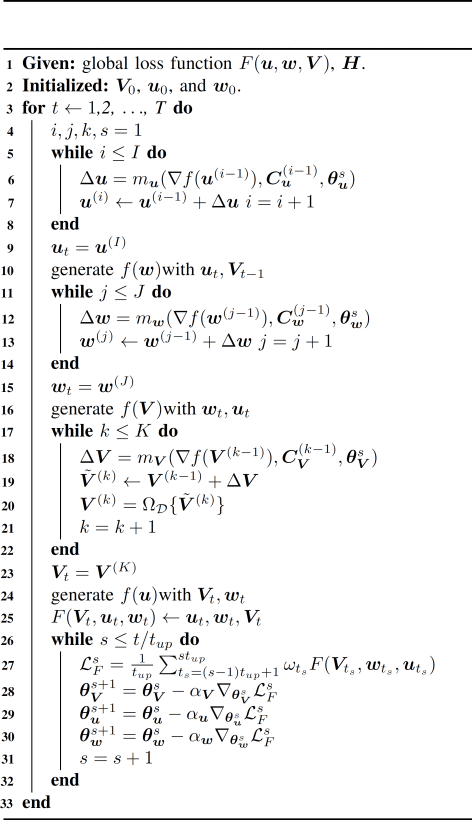
\includegraphics[width=3.25in]{assets/9518251-alg-1-source-large.png}%
\caption{Algorithm from \cite{LSTM_Net} for implementing the unfolded WMMSE algorithm using DNNs. Note that $m_u$, $m_w$, $m_V$ represent the neural networks for updating each variable respectively. Furthermore, $C_{u,w,V}$ represent the internal state of each cell for the respective parameter}%
\label{fig:LSTM_Algo}%
\end{figure}

The algorithm in figure \ref{fig:LSTM_Algo} shows the complete algorithm implemented by \cite{LSTM_Net} that was to be replicated and improved in this paper. Further discussion for the model will take place in the following section.

%-------------------------------------------------------------------------------
%                          Experimentation and Model
%-------------------------------------------------------------------------------
\section{Experimentation, Model, and Results}
The key stages for the planned experimentation was to first get a working comparison using the traditional WMMSE algorithm then to implement the design in \cite{LSTM_Net}, and then to exchange the LSTM modules with GRU modules and to do various testing of the hyper-parameters to observe the effects of using a different number of hidden layers. All of this was experimentation that \cite{LSTM_Net} did not perform and which would have revealed interesting new knowledge about applying DNNs in unsupervised learning optimization settings. Specifically, how much computation is actually required for the LSTM WMMSE algorithm to solve for beam-weights in wireless MISO systems. Several difficulties prevented this which will be discussed in some detail.

\subsection{PyTorch Implementation} 
Using the formulation of the problem in \ref{fig:LSTM_Algo}, the following graph shows the attempted implementation:

\begin{figure}[h]%
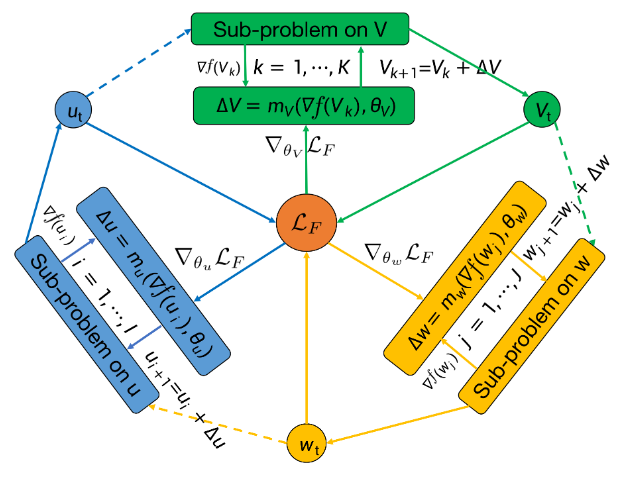
\includegraphics[width=3.25in]{assets/image-20231115093829461.png}%
\caption{The graph showing WMMSE implemented using RNNs for updating the values.}%
\label{fig:LSTM_Algo}%
\end{figure}

The unfolded LSTM WMMSE algorithm was implemented using a single class to contain all of the relevant parts so that everything would be self-contained in-order to facilitate future experimentation on various configurations. There were three individual LSTM networks, supporting variables, and an Adam optimizer for tuning the LSTM weights along with all the necessary helper functions to calculate the portions of the algorithm. More detail can be found in the code submission portion of this assignment which is thoroughly documented.

\subsection{WMMSE Deep Unfolding Replication}
The authors in \cite{Deep_Unfolding} made their code for the unfolded WMMSE algorithm public on GitHub which served as both a source of confusion and invaluable reference. The code provided by \cite{Deep_Unfolding} would have served as a benchmark to compare the performance of any simpler RNN on the beamforming problem. To this end, the results of the WMMSE algorithm were replicated and can be seen in Figure \ref{fig:WMMSE_ref}. Since much of the other code from \cite{Deep_Unfolding} used Tensorflow--which was unfamiliar--that part was not used. Unfortunately, since the results from \cite{LSTM_Net} could not be replicated with the details provided in their paper, no comparison was able to be performed.

\begin{figure}[h]%
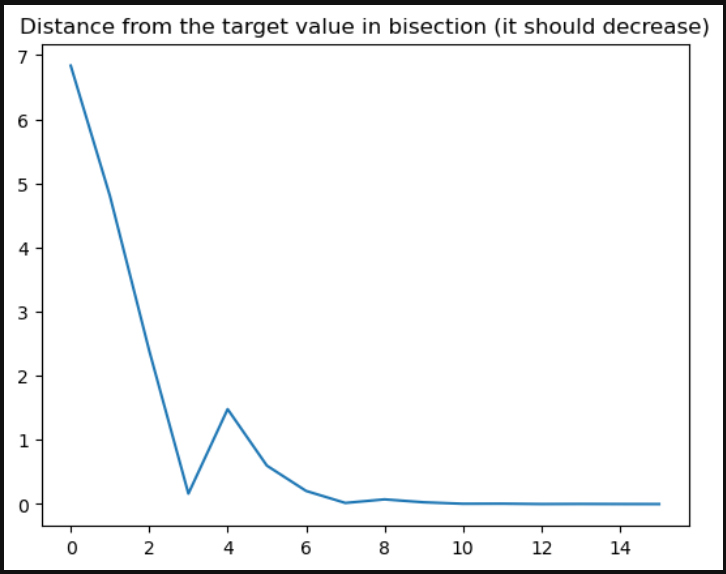
\includegraphics[width=3.25in]{assets/WMMSE_Working_Other_Peeps.png}%
\caption{WMMSE algorithm results implemented by \cite{Deep_Unfolding} showing the algorithm successfully converging to a solution. The code that generated this figure was copied from \cite{Deep_Unfolding} in order to be used as a basis of comparison.}%
\label{fig:WMMSE_Working}%
\end{figure}

Figure \ref{fig:WMMSE_Working} shows the WMMSE implementation by \cite{Deep_Unfolding} successfully solving for the beamweights in a 4 user 4 transmit antenna system. This was 

\subsection{Implementation Difficulties}
There were a number of substantial difficulties encountered when attempting to implement the algorithm described in \cite{LSTM_Net}. Ultimately, these difficulties prevented any additional analysis, but this section will explore them in detail in-place of novel results.

The first major difficulty encountered was related to the novel model type used in this project. All of the assignments this semester used supervised learning, so the challenges inherent to creating unsupervised models were novel and substantial. Learning how to make the PyTorch AutoGrad function ``happy'' was by far the most challenging. A particularly painful lesson was learning to detach old intermediate tensors after stepping the optimizer function. 

Implementing many of the update functions was difficult since many of them required ``in-place'' operations since many of the vectors were significantly dependent on position. For example, the error expectation vector, $e$ implemented as follows:

\begin{figure}[h]%
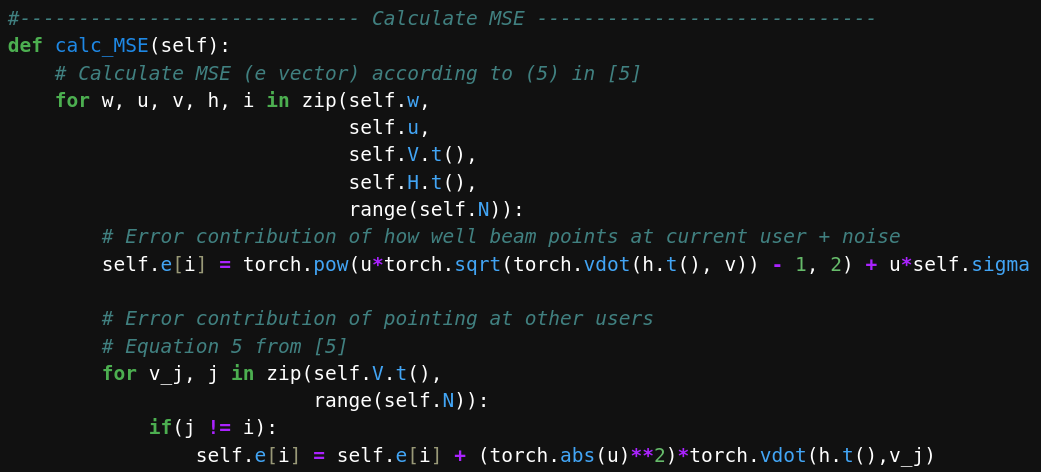
\includegraphics[width=3.25in]{assets/MSE_Algo.png}%
\caption{Calculating the Mean Squared Error vector for the neural network. Notice that many of the operations are ``in-place''. This is according to how MSE should be calculated to \cite{LSTM_Net}, but doing so has troublesome effects on the Autograd in PyTorch due to the in-place operations}%
\label{fig:LSTM_Algo}%
\end{figure}

I am still not sure that the gradient properly flows through this function, but did not have time to properly test it. I suspect that it does not, or that there are other errors in my implementation since the gradient diverges.

The second difficulty was massive uncertainty in implementation details of the algorithm. This was because the \cite{LSTM_Net} did not publish their code and were not very specific when describing which functions were used. This was further complicated by mistaking the code of \cite{Deep_Unfolding} for the LSTM module early on. The confusion this caused created major delays in development. After realizing this mistake, I did not have time to properly debug my algorithm implementation.

\subsection{Results}
After getting to a somewhat functional state, the LSTM network would always diverge. Many techniques were attempted to mitigate this from changing the initialization, to normalizing the inputs to the LSTMs, but nothing worked.

\begin{figure}[h]%
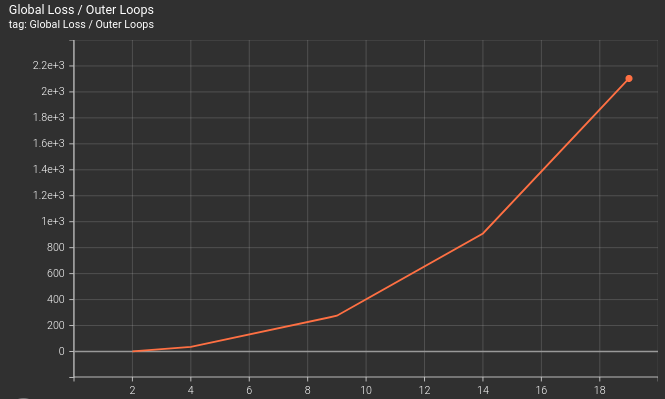
\includegraphics[width=3.25in]{assets/Exploding_Loss_Normalization.png}%
\caption{Diverging loss function of LSTM version of WMMSE}%
\label{fig:LSTM_Algo}%
\end{figure}

I then instrumented every part of the gradient to attempt to find the issue, but despite all my efforts, the gradient would not remain contained.

%-------------------------------------------------------------------------------
%                          Conclusion
%-------------------------------------------------------------------------------
\section{Conclusion}
Ultimately, I learned a large amount about implementing unsupervised learning algorithms using PyTorch. Specifically, how to make sure that the auto-gradients assemble properly. Unfortunately, because the implementation details were not specific enough, I was not able to successfully replicate the work of \cite{LSTM_Net}. This likely relates to my lack of training in optimization which likely would have made many of my questions self-evident. Eventually, I figured out an algorithm that I thought would be similar enough to the correct algorithm, but which clearly did not work. After I finally got the PyTorch autogradient to function, I was hit with a wall of diverging gradients, and despite attempting various initialization techniques, normalizing the gradient inputs to the LSTMs, I was not able to train a network to solve the optimization problem. Future work would focus on getting a working network to solve the algorithm, and re-working the helper functions to be transparent to the gradient function.  

\section{Roles}
Cameron Kramr was the sole member of this group and performed all roles.

\section{Code Availability}
\url{https://github.com/CameronKramr/ELEC_576_CKK5_Final_Project}

\nocite{*}
\bibliographystyle{plain}
\bibliography{references}

\end{document}
